\section{Fonctionnalités supplémentaires d'ADTool}
    \label{sec:ADTool}
    Cette section décrit la conception des fonctionnalités qui vont être ajoutées à ADTool afin de le rendre plus ergonomique.
    
    \subsection{Annulation des dernières actions}
    	La {\sc Figure}~{\ref{fig:ctrlz}} illustre l'agencement des classes permettant de réaliser la fonctionnalité d'annulation d'ADTool. Tout d'abord, chaque action annulable possède sa propre classe définissant l'action à exécuter, ainsi que l'action opposée permettant de l'annuler. Par exemple, les actions permettant d'ajouter un nœud-fils, de changer le label d'un nœud ou encore d'ajouter un paramètre possèdent leurs classes respectives \emph{AddChildEdit}, \emph{ChangeLabelEdit} et \emph{AddDomainEdit}. Ces dernières travaillent toutes sur un ADTree, représenté ici par une classe \emph{ADTree} pour simplifier le diagramme. Ces classes implémentent également \emph{UndoableEdit}, l'interface générique d'une action annulable. Enfin, un gestionnaire d'actions \emph{HistoryManager} stocke les actions effectuées dans un attribut, tout en disposant de méthodes permettant d'annuler ces actions dans l'ordre inverse de celui de leur réalisation.
    	
    	\begin{figure}[H]
	        \centering
	        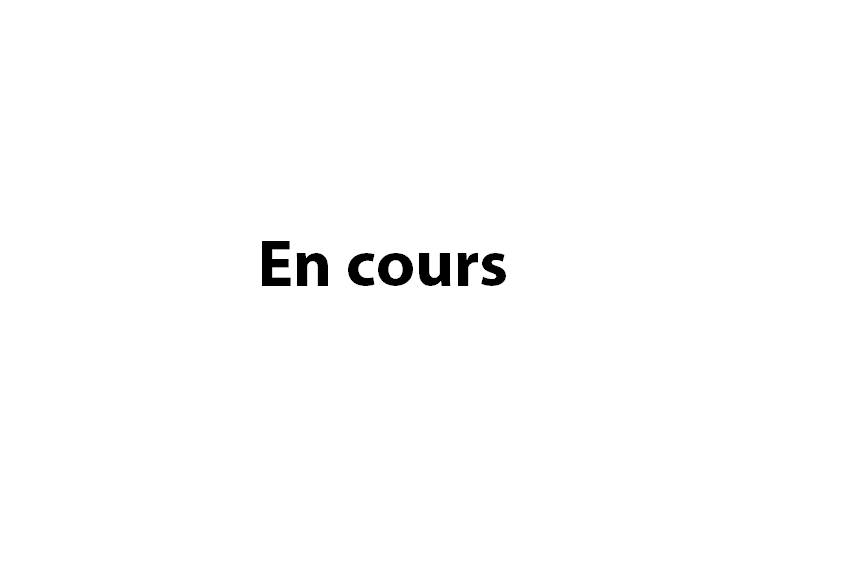
\includegraphics[height=0.8\textwidth]{figure/ctrlz.png}
	        \caption{Diagramme de classes de l'annulation des dernières actions.}
	        \label{fig:ctrlz}
	    \end{figure}
    
    \subsection{Couper-copier-coller}
		La {\sc Figure}~{\ref{fig:copiercoller}} illustre le diagramme de classes permettant de réaliser le couper-copier-coller d'ADTool. Les ADTrees, représentés par la classe \emph{ADTree}, implémentent \emph{Transferable}, l'interface permettant à un élément d'être coupé, copié ou collé. ADTool, schématisé par la classe \emph{ADTool}, se voit doté d'un \emph{ADTreeTransfertHandler}, une classe permettant de réaliser les actions couper-copier-coller en elles-mêmes. \emph{ADTreeTransfertHandler} implémente \emph{TransfertHandler}, l'interface qui permet de gérer un \og presse-papier \fg{}. Ce dernier est représenté par la classe \emph{Clipboard}, et contient l'élément coupé ou copié, c'est-à-dire un ADTree.
    	
    	\begin{figure}[H]
	        \centering
	        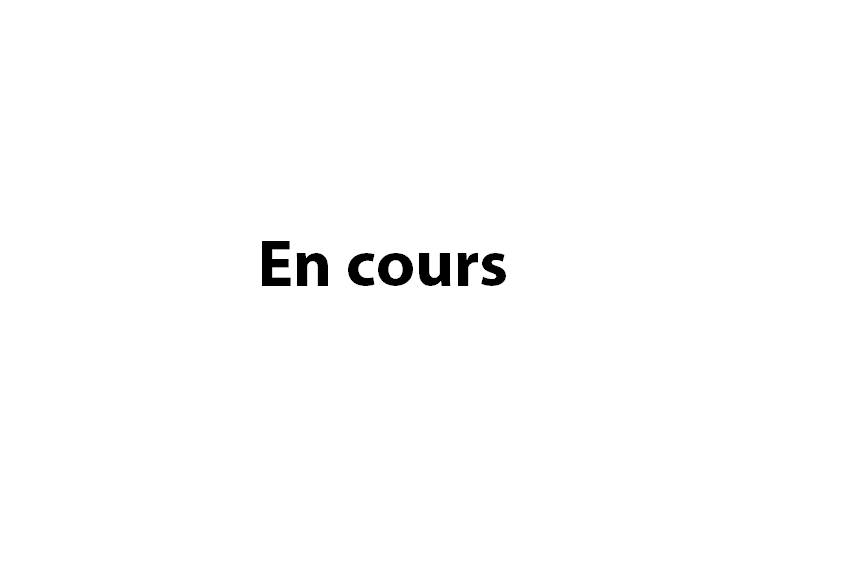
\includegraphics[height=0.6\textwidth]{figure/copiercoller.png}
	        \caption{Diagramme de classes du couper-copier-coller.}
	        \label{fig:copiercoller}
	    \end{figure}
	    
	\subsection{Vue globale des paramètres}
		À faire aussi
	
	\subsection{Amélioration de la représentation textuelle}
		À faire également
	  